\section{FDPBi  Class Reference}
\label{classFDPBi}\index{FDPBi@{FDPBi}}
A bidirectional version of forward dynamic programming. 


{\tt \#include $<$fdp.h$>$}

Inheritance diagram for FDPBi::\begin{figure}[H]
\begin{center}
\leavevmode
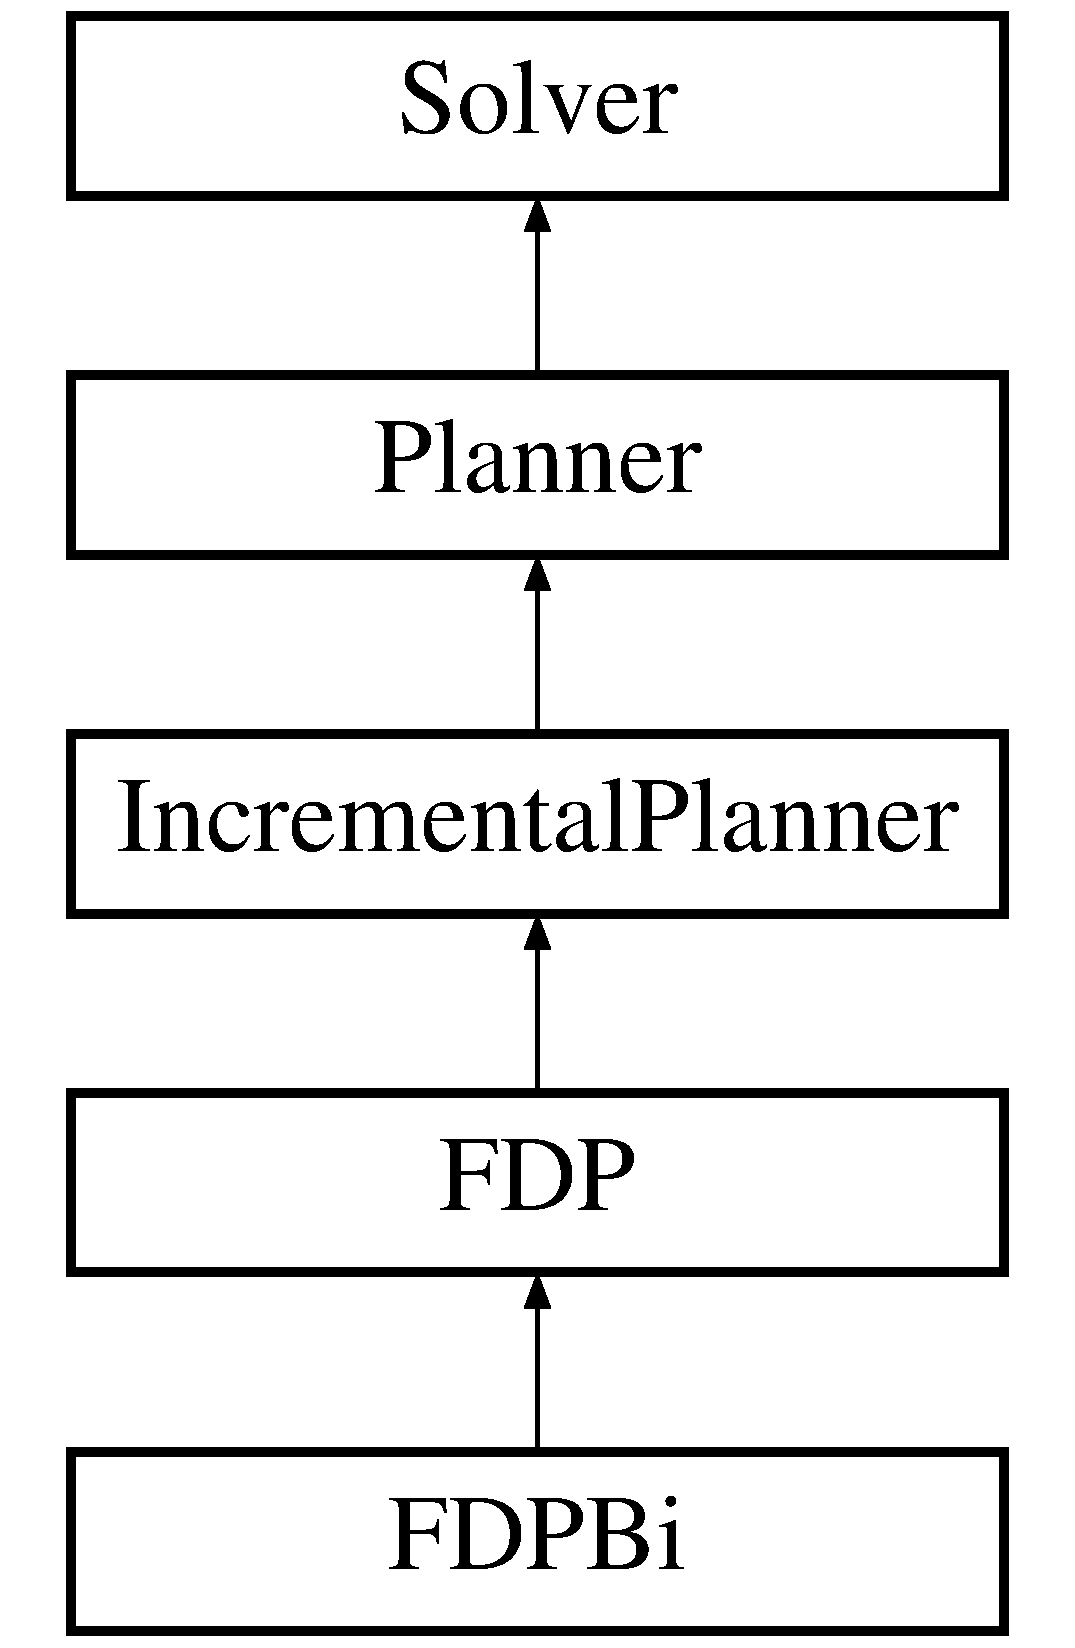
\includegraphics[height=5cm]{classFDPBi}
\end{center}
\end{figure}
\subsection*{Public Methods}
\begin{CompactItemize}
\item 
{\bf FDPBi} ({\bf Problem} $\ast$problem)
\begin{CompactList}\small\item\em A constructor that initializes data members.\item\end{CompactList}\item 
{\bf $\sim$FDPBi} ()
\begin{CompactList}\small\item\em Empty destructor.\item\end{CompactList}\item 
virtual void {\bf Reset} ()
\begin{CompactList}\small\item\em Reset the planner.\item\end{CompactList}\item 
virtual bool {\bf Plan} ()
\begin{CompactList}\small\item\em Attempt to solve an Initial-Goal query by growing an {\bf FDP} {\rm (p.\,\pageref{classFDP})}.\item\end{CompactList}\end{CompactItemize}
\subsection*{Protected Methods}
\begin{CompactItemize}
\item 
void {\bf Recover\-Solution} ({\bf MSLNode} $\ast$\&n1, {\bf MSLNode} $\ast$\&n2)
\begin{CompactList}\small\item\em Pull out the path and timings from the graphs.\item\end{CompactList}\end{CompactItemize}
\subsection*{Protected Attributes}
\begin{CompactItemize}
\item 
priority\_\-queue$<${\bf MSLNode}$\ast$,vector$<${\bf MSLNode}$\ast$$>$,{\bf MSLNode\-Greater}$>$ {\bf Q2}
\begin{CompactList}\small\item\em Priority queue of nodes.\item\end{CompactList}\end{CompactItemize}


\subsection{Detailed Description}
A bidirectional version of forward dynamic programming.



\subsection{Constructor \& Destructor Documentation}
\index{FDPBi@{FDPBi}!FDPBi@{FDPBi}}
\index{FDPBi@{FDPBi}!FDPBi@{FDPBi}}
\subsubsection{\setlength{\rightskip}{0pt plus 5cm}FDPBi::FDPBi ({\bf Problem} $\ast$ {\em problem})}\label{classFDPBi_a0}


A constructor that initializes data members.

\index{FDPBi@{FDPBi}!~FDPBi@{$\sim$FDPBi}}
\index{~FDPBi@{$\sim$FDPBi}!FDPBi@{FDPBi}}
\subsubsection{\setlength{\rightskip}{0pt plus 5cm}FDPBi::$\sim$FDPBi ()\hspace{0.3cm}{\tt  [inline]}}\label{classFDPBi_a1}


Empty destructor.



\subsection{Member Function Documentation}
\index{FDPBi@{FDPBi}!Plan@{Plan}}
\index{Plan@{Plan}!FDPBi@{FDPBi}}
\subsubsection{\setlength{\rightskip}{0pt plus 5cm}bool FDPBi::Plan ()\hspace{0.3cm}{\tt  [virtual]}}\label{classFDPBi_a3}


Attempt to solve an Initial-Goal query by growing an {\bf FDP} {\rm (p.\,\pageref{classFDP})}.



Reimplemented from {\bf FDP} {\rm (p.\,\pageref{classFDP_a3})}.\index{FDPBi@{FDPBi}!RecoverSolution@{RecoverSolution}}
\index{RecoverSolution@{RecoverSolution}!FDPBi@{FDPBi}}
\subsubsection{\setlength{\rightskip}{0pt plus 5cm}void FDPBi::Recover\-Solution ({\bf MSLNode} $\ast$\& {\em n1}, {\bf MSLNode} $\ast$\& {\em n2})\hspace{0.3cm}{\tt  [protected]}}\label{classFDPBi_b0}


Pull out the path and timings from the graphs.

\index{FDPBi@{FDPBi}!Reset@{Reset}}
\index{Reset@{Reset}!FDPBi@{FDPBi}}
\subsubsection{\setlength{\rightskip}{0pt plus 5cm}void FDPBi::Reset ()\hspace{0.3cm}{\tt  [virtual]}}\label{classFDPBi_a2}


Reset the planner.



Reimplemented from {\bf FDP} {\rm (p.\,\pageref{classFDP_a2})}.

\subsection{Member Data Documentation}
\index{FDPBi@{FDPBi}!Q2@{Q2}}
\index{Q2@{Q2}!FDPBi@{FDPBi}}
\subsubsection{\setlength{\rightskip}{0pt plus 5cm}priority\_\-queue$<$ {\bf MSLNode} $\ast$,vector$<$ {\bf MSLNode} $\ast$$>$,{\bf MSLNode\-Greater} $>$ FDPBi::Q2\hspace{0.3cm}{\tt  [protected]}}\label{classFDPBi_n0}


Priority queue of nodes.



The documentation for this class was generated from the following files:\begin{CompactItemize}
\item 
{\bf fdp.h}\item 
{\bf fdp.C}\end{CompactItemize}
